\subsection{Classical compressors on the full files}
\Cref{tab:full} gives the self-contained size of every classical method on the full TextBench files. Three groups separate cleanly. Order-0 entropy coders (Huffman, block-wise dynamic Huffman, rANS) stay between 3.6 and 6.0\,bpb, the order-0 entropy of the files. Dictionary and block-sorting compressors reach 0.6--4.2\,bpb, with bsc best on Hindi (\NumFBscHi{}\,bpb). Context models are best almost everywhere: zpaq's method~5 gives \NumFZpaqEn{}\,bpb on English sentences and \NumFZpaqXml{}\,bpb on \texttt{xml}. Chinese is the hardest text for every byte-level method (\NumFZpaqZh{}\,bpb at best), because each Han character spreads its information over three UTF-8 bytes whose statistics a byte context sees only partially.

\begin{table*}[t]\centering\caption{Compressed size in bits per byte on the full TextBench files (self-contained output, lower is better; best per column in bold; Canterbury: total of its eight text files). paq8px ran on xml and Canterbury only; neural and language-model methods are reported on 1\,MB slices in \cref{tab:slice}.}\label{tab:full}\small
\begin{adjustbox}{max width=\textwidth}\begin{tabular}{@{}clrrrrrrrr@{}}\toprule
Fam. & Method & English & Hindi & Chinese & enwik8 & dickens & xml & C/C++ & Canterbury\\\midrule
E & Huffman & 4.604 & 3.673 & 6.037 & 5.130 & 4.573 & 5.555 & 5.167 & 4.680\\
E & Dyn.\ Huffman & 4.608 & 3.675 & 6.039 & 5.134 & 4.578 & 5.564 & 5.177 & 4.766\\
E & rANS-0 & 4.582 & 3.643 & 6.002 & 5.100 & 4.533 & 5.510 & 5.140 & 4.648\\
E & Ext.\ Huffman & 9.095 & 5.083 & 9.188 & 8.710 & 9.072 & 4.192 & 7.064 & 8.412\\
E & EEHC & 9.132 & 5.094 & 9.229 & 8.750 & 9.112 & 4.201 & 7.071 & 8.464\\
\midrule
D & gzip & 3.285 & 1.721 & 4.233 & 2.951 & 3.026 & 0.986 & 1.427 & 2.966\\
D & bzip2 & 2.495 & 1.113 & 3.152 & 2.333 & 2.197 & 0.660 & 1.251 & 2.276\\
D & zstd & 2.430 & 1.136 & 3.123 & 2.234 & 2.236 & 0.678 & 1.135 & 2.582\\
D & xz & 2.405 & 1.109 & 3.064 & 2.176 & 2.222 & 0.651 & 1.083 & 2.549\\
D & Brotli & 2.399 & 1.144 & 3.079 & 2.164 & 2.220 & 0.644 & 1.081 & 2.460\\
D & bsc & 1.941 & \best{0.834} & 2.618 & 1.859 & 1.773 & 0.588 & 1.138 & 2.116\\
\midrule
M & PPMd & 1.963 & 1.160 & 2.575 & 1.895 & 1.803 & 0.743 & 1.219 & 2.054\\
M & zpaq & \best{1.833} & 1.035 & \best{2.495} & \best{1.673} & \best{1.644} & \best{0.489} & \best{0.822} & \best{1.992}\\
M & CM & 1.948 & 1.263 & 2.799 & 1.846 & 1.789 & 0.571 & 0.987 & 2.002\\
\bottomrule\end{tabular}\end{adjustbox}\end{table*}

\subsection{Neural and language-model compressors on 1\,MB slices}
\Cref{tab:slice} adds the slow methods on 1\,MB slices. Pretrained language models give the smallest payloads on all four slices they ran on. Qwen2.5-1.5B codes English sentences at \NumSQlEn{}\,bpb and Hindi at \NumSQlHi{}\,bpb; Qwen2.5-0.5B codes Chinese at \NumSQsZh{}\,bpb and enwik8 at \NumSQsWk{}\,bpb. The strongest classical model, paq8px, reaches \NumSPaqEn{}, \NumSPaqHi{}, \NumSPaqZh{} and \NumSPaqWk{}\,bpb on the same slices, so the best language model is \NumBestLLMgain{} smaller on \NumBestLLMfile{} and further ahead on English and enwik8. GPT-2 is a different story: it beats paq8px on English (\NumSGptEn{}) and enwik8 (\NumSGptWk{}) but loses badly on Hindi (\NumSGptHi{}) and Chinese (\NumSGptZh{}), where it is worse than bzip2.

The two online neural compressors do not reach PPM-class results at this size: TRACE gives \NumSTraceEn{}\,bpb on English and NNCP \NumSNncpEn{}\,bpb, both worse than PPMd (\NumSPpmdEn{}). Both start from random weights and learn while they code; one megabyte is too little for them to catch up with models whose statistics are counted directly. NNCP's published enwik9 results come from 1\,GB of training data and data-centre GPUs~\cite{bellard2021nncpv2}.

\begin{table*}[t]\centering\caption{Bits per byte on the 1\,MB slices, all methods (self-contained output; language-model rows exclude the model weights, see \cref{tab:cost}). \na: not run.}\label{tab:slice}\small
\begin{adjustbox}{max width=\textwidth}\begin{tabular}{@{}clrrrrrrr@{}}\toprule
Fam. & Method & English & Hindi & Chinese & enwik8 & dickens & xml & C/C++\\\midrule
E & Huffman & 4.605 & 3.761 & 6.219 & 5.087 & 4.540 & 5.370 & 5.266\\
E & Dyn.\ Huffman & 4.620 & 3.780 & 6.229 & 5.106 & 4.558 & 5.396 & 5.289\\
E & rANS-0 & 4.581 & 3.733 & 6.189 & 5.062 & 4.502 & 5.348 & 5.238\\
E & Ext.\ Huffman & 8.410 & 3.586 & 9.543 & 7.946 & 7.710 & 3.620 & 6.341\\
E & EEHC & 8.462 & 3.614 & 9.607 & 7.993 & 7.753 & 3.649 & 6.375\\
\midrule
D & gzip & 3.324 & 1.800 & 4.267 & 2.846 & 2.960 & 1.071 & 1.727\\
D & bzip2 & 2.559 & 1.190 & 3.201 & 2.251 & 2.162 & 0.784 & 1.503\\
D & zstd & 2.769 & 1.410 & 3.531 & 2.401 & 2.381 & 0.908 & 1.455\\
D & xz & 2.731 & 1.383 & 3.434 & 2.326 & 2.356 & 0.885 & 1.397\\
D & Brotli & 2.631 & 1.395 & 3.413 & 2.248 & 2.317 & 0.867 & 1.378\\
D & bsc & 2.277 & 1.067 & 2.954 & 2.034 & 1.913 & 0.715 & 1.362\\
\midrule
M & PPMd & 2.232 & 1.247 & 2.906 & 2.000 & 1.879 & 0.829 & 1.375\\
M & zpaq & 2.170 & 1.188 & 2.843 & 1.840 & 1.781 & 0.671 & 1.079\\
M & CM & 2.173 & 1.187 & 2.860 & 1.922 & 1.852 & 0.703 & 1.220\\
M & paq8px & 1.957 & 0.939 & 2.590 & 1.555 & \best{1.589} & \best{0.552} & \best{0.802}\\
M & TRACE & 2.777 & 1.464 & 3.442 & 2.600 & 2.407 & 1.050 & 2.026\\
M & NNCP & 2.830 & 1.405 & 3.444 & \na & \na & \na & \na\\
\midrule
L & GPT-2 & 1.250 & 1.557 & 3.246 & 1.211 & \na & \na & \na\\
L & Qwen-0.5B & 1.087 & 0.878 & \best{1.635} & \best{0.875} & \na & \na & \na\\
L & Qwen-1.5B & \best{0.979} & \best{0.770} & \na & \na & \na & \na & \na\\
\bottomrule\end{tabular}\end{adjustbox}\end{table*}

\subsection{What the decoder must hold}\label{sec:costres}
\Cref{tab:cost} charges each method for its pretrained knowledge, and \cref{fig:breakeven} plots the result against input size. The payload of Qwen-0.5B is \NumQsEnrP{}--\NumQsHirP{}\,bpb on English and Hindi, but its \NumQwenSmallGB{}\,GB of weights make its rate about 9\,bpb at 1\,GB of input; it overtakes xz only after \NumBreakEvenSmall{} of text, and paq8px only after \NumBreakEvenSmallPaq{}. For Qwen-1.5B (\NumQwenLargeGB{}\,GB) the break-even points are \NumBreakEvenLarge{} and \NumBreakEvenLargePaq{}. GPT-2 never repays its weights against paq8px on these texts, because it loses on Hindi and Chinese. At the other end of the scale, Brotli's 122\,KB built-in dictionary is repaid after \NumBreakEvenBrotli{}. The Huffman-family coders show the opposite pattern on the payload column: EEHC's payload alone is \NumEEHCpayloadMean{}\,bpb averaged over the full files, better than gzip, but its decodable file averages \NumEEHCfileMean{}\,bpb (\cref{sec:huff}).

\begin{table}[t]\centering\caption{Three cost levels on the English, Hindi, Chinese and enwik8 slices (bits per byte, mean over the slices; Qwen-1.5B: English and Hindi only): payload $r_P$, self-contained file $r_F$, and $r_K$ with the pretrained knowledge charged once on 1\,GB or 1\,TB of input. $N^\ast$: input size at which that knowledge is paid back against xz and against paq8px on the same slices.}\label{tab:cost}\footnotesize\setlength{\tabcolsep}{3.5pt}
\begin{adjustbox}{max width=\columnwidth}\begin{tabular}{@{}lrrrrrr@{}}\toprule
Method & $r_P$ & $r_F$ & $r_K$@1GB & $r_K$@1TB & $N^\ast_{\mathrm{xz}}$ & $N^\ast_{\mathrm{paq8px}}$\\\midrule
Huffman & 4.915 & 4.918 & 4.918 & 4.918 & -- & --\\
Dyn.\ Huffman & 4.934 & 4.934 & 4.934 & 4.934 & -- & --\\
rANS-0 & 4.891 & 4.891 & 4.891 & 4.891 & -- & --\\
Ext.\ Huffman & 1.949 & 7.371 & 7.371 & 7.371 & -- & --\\
EEHC & 1.996 & 7.419 & 7.419 & 7.419 & -- & --\\
gzip & 3.059 & 3.059 & 3.059 & 3.059 & -- & --\\
bzip2 & 2.300 & 2.300 & 2.300 & 2.300 & -- & --\\
zstd & 2.528 & 2.528 & 2.528 & 2.528 & -- & --\\
xz & 2.468 & 2.468 & 2.468 & 2.468 & -- & --\\
Brotli & 2.422 & 2.422 & 2.423 & 2.422 & 21.0\,MB & never\\
bsc & 2.083 & 2.083 & 2.083 & 2.083 & -- & --\\
PPMd & 2.096 & 2.096 & 2.096 & 2.096 & -- & --\\
zpaq & 2.010 & 2.010 & 2.010 & 2.010 & -- & --\\
CM & 2.036 & 2.036 & 2.036 & 2.036 & -- & --\\
paq8px & 1.760 & 1.760 & 1.760 & 1.760 & -- & --\\
TRACE & 2.571 & 2.571 & 2.571 & 2.571 & -- & --\\
NNCP & 2.560 & 2.560 & 2.560 & 2.560 & -- & --\\
GPT-2 & 1.805 & 1.816 & 6.201 & 1.820 & 6.7\,GB & never\\
Qwen-0.5B & 1.112 & 1.119 & 9.023 & 1.127 & 5.9\,GB & 12.3\,GB\\
Qwen-1.5B & 0.868 & 0.875 & 25.574 & 0.899 & 20.9\,GB & 43.1\,GB\\
\bottomrule\end{tabular}\end{adjustbox}\end{table}

\begin{figure}[t]\centering
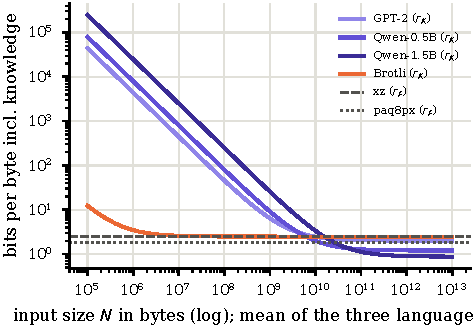
\includegraphics[width=\columnwidth]{breakeven}
\caption{Rate including pretrained knowledge, $r_K(N)$, against input size $N$ (mean of the three language slices). Horizontal lines: self-contained rate of xz and paq8px on the same slices.}
\label{fig:breakeven}
\end{figure}

\subsection{Script and tokeniser}\label{sec:scriptres}
\Cref{tab:tok} splits each language model's payload into tokens per byte and bits per token, and \cref{fig:languages} compares the methods across scripts. On English the two tokenisers produce the same number of tokens (\NumGptEntpb{} and \NumQsEntpb{} per byte), so the whole difference between GPT-2 and Qwen-0.5B (\NumGptEnrP{} vs \NumQsEnrP{}\,bpb) is prediction: \NumGptEnbpt{} against \NumQsEnbpt{} bits per token. On Hindi, GPT-2's tokeniser emits \NumGptHitpb{} tokens per byte against Qwen's \NumQsHitpb{}, while the bits per token are close (\NumGptHibpt{} and \NumQsHibpt{}); on a logarithmic scale the token count accounts for \NumTokShareHi{} of the gap. On Chinese GPT-2 needs \NumGptZhtpb{} tokens per byte against \NumQsZhtpb{}; the token count alone accounts for more than the entire gap (\NumTokShareZh{}), because Qwen's longer tokens each carry more information (\NumQsZhbpt{} bits). Holding the tokeniser fixed, tripling the model from 0.5B to 1.5B parameters lowers the payload by \NumScaleEn{} on English and \NumScaleHi{} on Hindi.

Bits per byte flatter scripts with multi-byte characters. Per character, Qwen-0.5B spends \NumQsEnbpcV{} bits on English, \NumQsHibpcV{} on Hindi and \NumQsZhbpcV{} on Chinese (\cref{tab:tok}); the Leipzig files are not translations of each other, so these figures compare scripts, not languages.

\begin{table}[t]\centering\caption{Language-model payload rate split into tokens per byte (tokeniser) and bits per token (prediction): $r_P=(T/N)(8P/T)$; also bits per character and per line (one sentence per line in the Leipzig files). No piece needed the raw fallback.}\label{tab:tok}\footnotesize\setlength{\tabcolsep}{3.5pt}
\begin{adjustbox}{max width=\columnwidth}\begin{tabular}{@{}llrrrrr@{}}\toprule
Model & Text & Tok./byte & Bits/tok. & $r_P$ & Bits/char & Bits/line\\\midrule
GPT-2 & English & 0.217 & 5.74 & 1.246 & 1.25 & 164\\
GPT-2 & Hindi & 0.596 & 2.59 & 1.542 & 3.90 & 394\\
GPT-2 & Chinese & 0.690 & 4.68 & 3.229 & 8.00 & 329\\
GPT-2 & enwik8 & 0.286 & 4.21 & 1.204 & 1.21 & 103\\
\midrule
Qwen-0.5B & English & 0.219 & 4.95 & 1.083 & 1.08 & 143\\
Qwen-0.5B & Hindi & 0.364 & 2.39 & 0.870 & 2.20 & 222\\
Qwen-0.5B & Chinese & 0.273 & 5.96 & 1.627 & 4.03 & 166\\
Qwen-0.5B & enwik8 & 0.264 & 3.29 & 0.869 & 0.87 & 75\\
\midrule
Qwen-1.5B & English & 0.219 & 4.46 & 0.975 & 0.98 & 129\\
Qwen-1.5B & Hindi & 0.364 & 2.09 & 0.761 & 1.92 & 195\\
\bottomrule\end{tabular}\end{adjustbox}\end{table}

\begin{figure*}[t]\centering
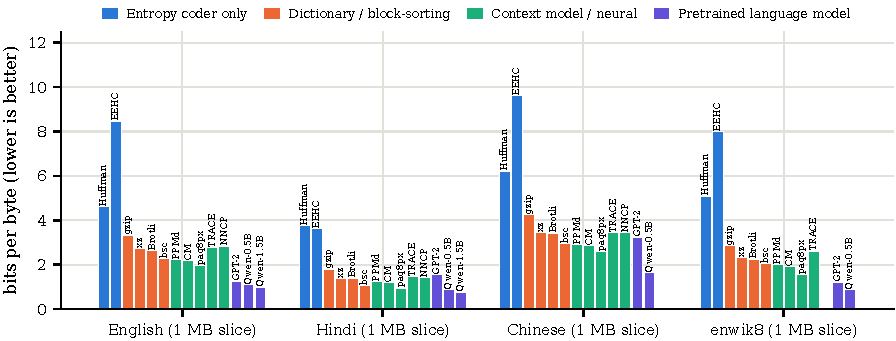
\includegraphics[width=\textwidth]{languages}
\caption{Bits per byte on the 1\,MB slices of English, Hindi, Chinese and enwik8, by method family. Labels name each bar's method.}
\label{fig:languages}
\end{figure*}

\subsection{Huffman-family coders}\label{sec:huff}
Plain order-0 Huffman coding stays within \NumHuffOverHzeroMax\% of the order-0 entropy on every file, and rANS, which is not limited to whole bits per symbol, is \NumRansUnderHuff\% smaller on average (\cref{tab:full}). Rebuilding the tree every 4\,KiB from the bytes seen so far (block-wise dynamic Huffman~\cite{klein2024dynhuff}) costs at most \NumDynOverStaticMax\% against static Huffman and needs no stored table. Coding blocks instead of bytes, as Extended Huffman and EEHC do, helps only when whole blocks repeat: of the \NumEEHCfiles{} full files, EEHC's decodable output is larger than order-0 Huffman's on \NumEEHCworseThanHuffman{}, and only the highly repetitive \texttt{xml} benefits (\NumFEehcXml{} vs \NumFHufXml{}\,bpb). On English sentences EEHC's file is larger than the input (\NumFEehcEn{}\,bpb), even though its payload alone is \NumEEHCpayloadEn{}\,bpb. The base-8 tree adds up to \NumBaseEightMax\% over a binary tree on the same blocks, as expected: a binary Huffman code is optimal in bits, and any base-8 code is a binary code with 3 bits per digit.

\subsection{Speed and memory}
\Cref{fig:speed} places each method by compression speed and mean rate on the slices. The cost of the last bits is steep: zstd and Brotli run at megabytes per second, PPMd and bsc remain fast, zpaq and our CM coder run at hundreds of kilobytes per second, and paq8px, NNCP, TRACE and the language models fall to kilobytes per second in both directions, since every one of them decodes by repeating the encoder's computation. paq8px at level~9 also needs 4.3\,GB of memory, and the language models need a GPU.

\begin{figure}[t]\centering
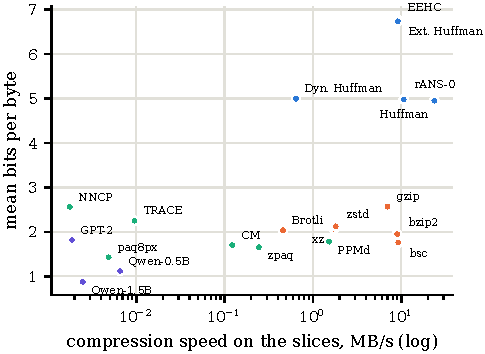
\includegraphics[width=\columnwidth]{speed}
\caption{Compression speed (log scale) against mean bits per byte on the 1\,MB slices. Colours as in \cref{fig:languages}.}
\label{fig:speed}
\end{figure}
